% \documentclass{article}
% % Define color and JSON style for listings
% \usepackage[preprint]{neurips_2025}
% \usepackage[most]{tcolorbox}
% \usepackage{listings}
% \usepackage{float}
% \usepackage{booktabs}
% \usepackage{array}
% \usepackage{hyperref}
% \usepackage{graphicx}
% \usepackage{xcolor}
% \usepackage{subcaption}
% \usepackage{placeins}

% \definecolor{lightgray}{gray}{0.95}
% \lstdefinestyle{json}{
%   backgroundcolor=\color{lightgray},
%   basicstyle=\ttfamily\small,
%   breaklines=true,
%   frame=single,
%   showstringspaces=false
% }
% \begin{document}

\section{Technical Appendices}
\subsection{Code and Data Availability}
All code and data necessary for replicating experiments can be accessed here: \url{https://anonymous.4open.science/r/phate-for-text-4D7D/README.md}. 
\subsection{Parameter Selection Process}
\label{subsec:parameters}
Parameter selection for both the dimensionality reduction and clustering followed a progressive refinement strategy. We explored a broad range of parameter combinations. Each combination of method and parameters was evaluated on the smaller synthetic datasets to assess baseline performance.

\begin{table*}[ht]
\centering
\caption{Initial parameters for dimensionality reduction and clustering}
\begin{tabular}
{@{}lp{10cm}@{}}
\toprule
\textbf{Method} & \textbf{Parameters} \\ \midrule
UMAP & \texttt{n\_components: [100, 300], min\_dist: [0.05, 0.1, 0.2, 0.3, 0.4, 0.5], n\_neighbors: [5, 10, 15, 25]} \\ \midrule
PCA & \texttt{n\_components: [100, 300]} \\ \midrule
PHATE & \texttt{n\_components: [100, 300], decay: [10, 20, 40], t: [7, 11, auto], knn: [3, 5, 7]} \\ \midrule
HDBSCAN & \texttt{cluster\_selection\_epsilon: [0, 0.1, 0.01, 0.001], cluster\_selection\_method: [eom, leaf]} \\ \midrule
Agglomerative clustering & \texttt{linkage: [ward, average]} \\ \midrule
Diffusion condensation & \texttt{k: [4, 5, 10], t: [3, 10, 30], alpha: [2, 4, 8], bandwidth\_norm: [max, l1]} \\
\bottomrule
\end{tabular}
\end{table*}

% \begin{table}[H]
% \centering
% \caption{Initial parameters for dimensionality reduction and clustering}
% \begin{tabular}{@{}lp{7cm}@{}}
% \toprule
% \textbf{Method} & \textbf{Parameters} \\ \midrule
% UMAP & 
% \begin{tabular}[t]{@{}l@{}}
% \texttt{n\_components: [100, 300],} \\
% \texttt{min\_dist: [0.05, 0.1, 0.2, 0.3, 0.4, 0.5],} \\
% \texttt{n\_neighbors: [5, 10, 15, 25]}
% \end{tabular} \\ \midrule
% PCA & 
% \texttt{n\_components: [100, 300]} \\ \midrule
% PHATE & 
% \begin{tabular}[t]{@{}l@{}}
% \texttt{n\_components: [100, 300], decay: [10, 20, 40],} \\
% \texttt{t: [7, 11, auto], knn: [3, 5, 7]}
% \end{tabular} \\ \midrule
% HDBSCAN & 
% \begin{tabular}[t]{@{}l@{}}
% \texttt{cluster\_selection\_epsilon: [0, 0.1, 0.01, 0.001],} \\
% \texttt{cluster\_selection\_method: [eom, leaf]}
% \end{tabular} \\ \midrule
% Agglomerative clustering & 
% \texttt{linkage: [ward, average]} \\ \midrule
% Diffusion condensation & 
% \begin{tabular}[t]{@{}l@{}}
% \texttt{k: [4, 5, 10], t: [3, 10, 30],} \\
% \texttt{alpha: [2, 4, 8], bandwidth\_norm: [max, l1]}
% \end{tabular} \\
% \bottomrule
% \end{tabular}
% \end{table}

We evaluated performance using both random forest classifiers and simple averaging metrics to identify high-performing parameter configurations. For the random forest we used the parameters as predictors and average ARI as the target. Based on these results, we reduced the search space and standardized the dimensionality parameter $\mathtt{n\_components}$ to values of 100 and 300 across all dimensionality reduction methods.
\begin{table*}[ht]
\centering
\caption{Refined parameters for larger synthetic datasets}
\begin{tabular}{@{}lp{10cm}@{}}
\toprule
\textbf{Method} & \textbf{Parameters} \\ \midrule
UMAP & \texttt{n\_components: [100, 300], min\_dist: [0.05, 0.1], n\_neighbors: [10, 15]} \\ \midrule
PCA & \texttt{n\_components: [100, 300]} \\ \midrule
PHATE & \texttt{n\_components: [100, 300], decay: [20], t: [auto]} \\ \midrule
HDBSCAN & \texttt{cluster\_selection\_epsilon: [0, 0.001], cluster\_selection\_method: [eom]} \\ \midrule
Agglomerative clustering & \texttt{linkage: [ward]} \\ \midrule
Diffusion condensation & \texttt{k: [5, 10], t: [3, 10], alpha: [4], bandwidth\_norm: [max]} \\ 
\bottomrule
\end{tabular}
\end{table*}

Parameters were selected on the basis of best mean performance from the previous step. $\mathtt{n\_components}$ was universally chosen as 300.  
\begin{table*}[ht]
\centering
\caption{Final parameters for largest and real-world datasets}
\begin{tabular}{@{}lp{10cm}@{}}
\toprule
\textbf{Method} & \textbf{Parameters} \\ \midrule
UMAP & \texttt{n\_components: [300], min\_dist: [0.05], n\_neighbors: [10]} \\ \midrule
PCA & \texttt{n\_components: [300]} \\ \midrule
PHATE & \texttt{n\_components: [300], decay: [20], t: [auto]} \\ \midrule
HDBSCAN & \texttt{cluster\_selection\_epsilon: [0], cluster\_selection\_method: [eom]} \\ \midrule
Agglomerative clustering & \texttt{linkage: [ward]} \\ \midrule
Diffusion condensation & \texttt{k: [10], t: [3], alpha: [4], bandwidth\_norm: [max]} \\
\bottomrule
\end{tabular}
\label{tab:final-parameters}
\end{table*}

UMAP parameters selected on the basis of hierarchical clustering did not produce desirable visualizations. % This is partially due to visualizing with the top 2 coordinates with \texttt{n\_components=300}. 
Hence, to ensure a fair visual comparison with PHATE in particular, the second-best configuration of UMAP parameters (Table \ref{tab:UMAP-viz})  were used for the generated data visualizations in the results. %The default parameters had emerged as the second-best configuration via the hierarchical clustering evaluation. This adjustment was made solely for visualization purposes and does not affect the integrity of the main comparative analysis.
In the interest of transparency, we have also included the plots generated using the best-performing parameter set (as listed in Table \ref{tab:final-parameters}) in Figure \ref{fig:UMAP-alt} for reference. For completeness, we also include visualizations of the data sets with default parameter settings for PHATE and UMAP in Figure \ref{fig:default-visuals} (we did not vary PCA or t-SNE  parameters that affect 2-D visualization).  %The fact that the best-performing hierarchical clustering parameters for PHATE also produced informative visualizations speaks to the robustness of the method for visualizing textual data.

\begin{table*}[ht]
\centering
\caption{UMAP parameters used only for generated data visualizations.}
\begin{tabular}{@{}lp{10cm}@{}}
\toprule
\textbf{Method} & \textbf{Parameters} \\ \midrule
UMAP (visualization only) & \texttt{n\_components: [300], min\_dist: [0.1], n\_neighbors: [15]} \\
\bottomrule
\end{tabular}
\label{tab:UMAP-viz}
\end{table*}

\begin{figure*}[ht]
    \centering
    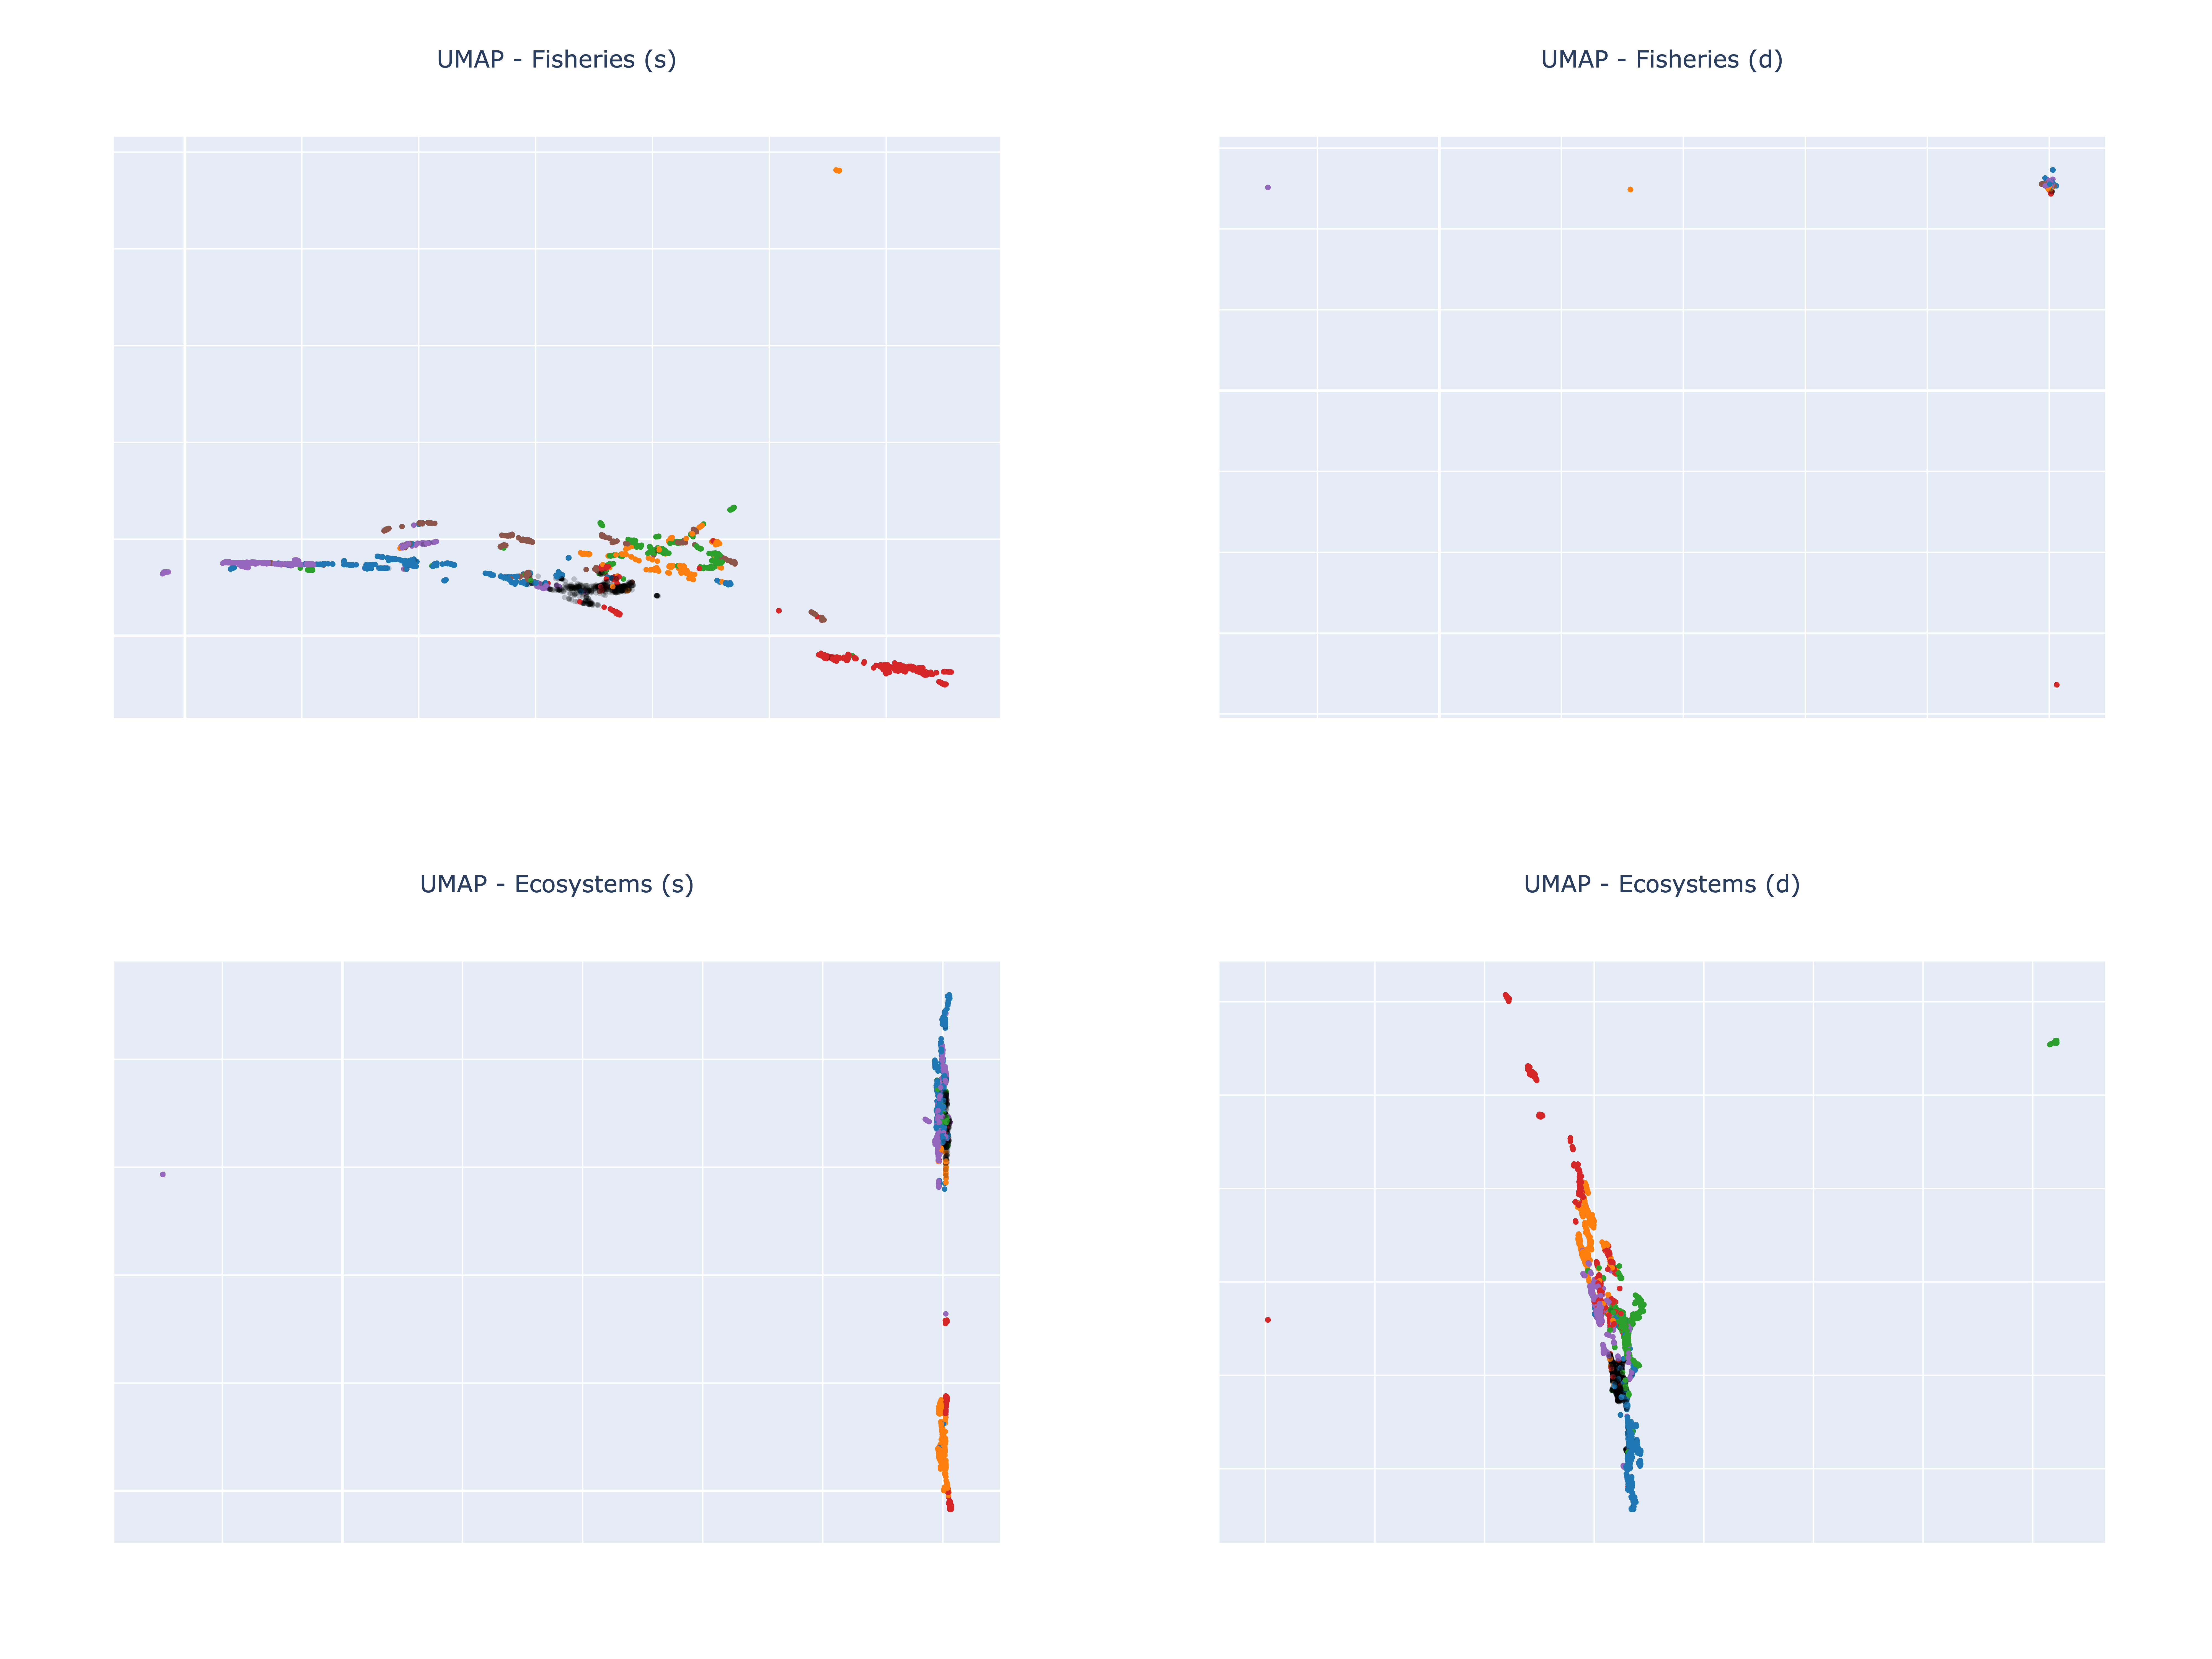
\includegraphics[width=1\linewidth]{UMAP_alternate_params.png}
    \caption{UMAP visualizations of generated data using top-performing clustering parameters}
    \label{fig:UMAP-alt}
\end{figure*}  

\begin{figure*}[ht]
    \centering
    \includegraphics[width=.9\linewidth,keepaspectratio=true]{all_embeddings_subplot_defaults.png}
    \caption{UMAP and PHATE embeddings visuals with default parameters}
    \label{fig:default-visuals}
\end{figure*}  

\subsection{Example GPT Query Prompt and Response}
\subsubsection*{System and user prompt}
In this example, the \textbf{Parent Topic} is the direct parent, while the \textbf{Core Topic} is the highest-level topic in the hierarchy.

% \begin{tcolorbox}[title=System and User Prompt, colback=gray!5, colframe=gray!40!black, boxrule=0.5pt, breakable=unlimited]
\begin{lstlisting}[style=json]
[
  {
    "role": "system",
    "content": "You generate hierarchical topic structures and maintain consistency across responses.
    - Subtopics must be distinct and separate from one another.
    - Subtopics must be more specific than the parent but still general.
    - Each subtopic must be measurable in magnitude (able to increase or decrease, but does not include whether it is an increase or decrease).
    - You have flexibility to generate fewer subtopics if meaningful distinctions become unclear.
    - Subtopics should not describe change itself (e.g., 'fluctuation in X'), but rather be the thing that changes.
    - Subtopics should not merely influence the parent topic but be a sub-example or more specific application of the parent."
  }
]
...
\end{lstlisting}
% \end{tcolorbox}

Expand the given Parent Topic into a list of up to 5 or fewer specific subtopics that:
- Are related to Economic Impact Metrics, especially Economic Impact Metrics.
- Clearly reflect their connection to the Parent Topic and Core Topic through their nature and scope.
- Are Not related to the other core topics: [].
- Much Less related to sibling topics: [].
- Fit within the given theme: Energy, Ecosystems, and Humans.
- Each subtopic should be a subcategory of the parent topic, such that a change in the subtopic implies a change in the broader topic.

Parent Topic: Renewable Energy Investment 
Core Topic: Economic Impact Metrics

Output Format: A JSON list of up to 5 subtopics, e.g.:

["Subtopic 1", "...", "Subtopic 5"]


\subsubsection*{Generated output}

...

% \begin{tcolorbox}[title=Model Output, colback=gray!5, colframe=gray!40!black, boxrule=0.5pt]
\begin{lstlisting}[style=json]
  [
    "Job Creation in Renewable Sector",
    "Capital Expenditure on Green Technologies",
    "Subsidies for Renewable Energy Projects",
    "Grid Infrastructure Upgrades for Renewables",
    "R&D Investment in Renewable Technologies"
  ]
  \end{lstlisting}
  % \end{tcolorbox}
\subsection{Dataset Details}
We evaluated our method on three publicly available datasets, each containing hierarchical categorical labels. Below, we detail the preprocessing, embedding, and clustering procedures applied to each dataset.

\subsubsection*{Amazon Product Reviews}

This dataset is derived from Amazon product reviews. Each entry includes a product \texttt{Title} and three hierarchical category levels (i.e., \texttt{Cat1}, \texttt{Cat2}, \texttt{Cat3}). We used the product title as the input text for embedding. The three category levels served as the hierarchical ground truth for evaluating the clustering quality. This dataset allowed us to analyze how product titles align with categorical hierarchies in a consumer retail context.

\subsubsection*{DBpedia}

For the purposes of embedding and visualization, we processed the text from the train, validation, and test splits. We used the textual description fields as input for embedding and dimensionality reduction. Clustering evaluation was then performed on the test set using the provided hierarchical labels (\texttt{l1}, \texttt{l2}, \texttt{l3}) as the categorical hierarchy.

\subsubsection*{Web of Science}

For each paper in the Web of Science (WOS) corpus, we used the provided keywords as the textual input for embedding and reduction. We then performed clustering on the resulting representations. Hierarchical labels were derived from the \texttt{Domain} and \texttt{area} fields, which represent high-level and mid-level classifications respectively. These served as the ground truth for evaluating the clustering performance.
\subsubsection*{arXiv}

The arXiv dataset contains approximately 30,000 scientific documents constructed from titles and abstracts. Documents were filtered to relevant domains and used to form a unified textual representation. Hierarchical ground truth labels were derived from subject categories at two levels (L1 and L2). Embeddings were generated using \texttt{all-MiniLM-L6-v2} and \texttt{Qwen3-Embedding-0.6B}.

\subsubsection*{RCV1}
The RCV1 dataset consists of news articles annotated with hierarchical topic codes. We used a processed subset where each document combines headline and body text. Ground truth labels were derived from Reuters topic codes, forming a hierarchical structure. Embeddings were generated using both \texttt{all-MiniLM-L6-v2} and \texttt{Qwen3-Embedding-0.6B}, and the same dimensionality reduction and clustering pipeline was applied as in the arXiv experiments.


\subsubsection*{Environmental Protection Agency (EPA)}
Comments were obtained from the federal register through Mirrulations\footnote{https://registry.opendata.aws/mirrulations/}. Comments were filtered to include only those relevant to the EPA. Standard pre-processing steps were applied, including removal of stop-words, HTML tags, and punctuation. Very short comments (<10 characters) were discarded, and long comments (>512 tokens) were truncated using a head-tail strategy (first and last 25\%). Only comments submitted after 2000 were retained. Sentence embeddings were generated using the Sentence-BERT model \texttt{all-MiniLM-L6-v2}.
% Across all datasets, we applied consistent embedding and dimensionality reduction techniques before performing clustering. Hierarchical clustering quality was assessed using the corresponding multi-level categorical labels, with particular emphasis on the test set where applicable.

\subsection{Hardware and runtime environment}
\begin{itemize}
  \item \textbf{Device:} Apple MacBook Pro 16-inch
  \item \textbf{Chip:} Apple M3 Max
  \item \textbf{CPU Cores:} 16-core CPU (12 performance cores, 4 efficiency cores)
  \item \textbf{GPU:} Not used for the majority of experiments
  \item \textbf{RAM:} 64 GB
  \item \textbf{Purpose:} All experiments, including data generation and evaluation, were conducted locally on this machine.
  \item \textbf{Runtime Summary:}
  \begin{itemize}
    \item Data generation tasks were completed in approximately 1 hour for the largest datasets.
    \item The parameter search for generated datasets took under 72 hours in total.
    \item Evaluation on DBpedia completed in 24 hours.
    \item The evaluations on Amazon and Web of Science were completed in less than 6 hours each.
  \end{itemize}
  % \item \textbf{Dataset Evaluation Pipeline:}
  % \begin{itemize}
  %   \item All data sets were embedded using GPT-based representations.
  %   \item Dimensionality reduction was performed using UMAP, PHATE, t-SNE, and PCA.
  %   \item Each reduced data set was clustered using Agglomerative Clustering, HDBSCAN, and Diffusion Condensation.
  %   \item Clustering was also performed on the raw text embeddings of the generated (synthetic) data sets.
  % \end{itemize}
  
\end{itemize}


% \end{document}